We examine three training-time signals logged to W\&B at every step across all four pre-P3 runs (467 steps each).

\paragraph{Mean reward curves.}
Figure~\ref{fig:p4-reward-curves} shows the total mean reward per step.
All runs exhibit a sharp initial improvement followed by a decline toward the starting level, consistent with REINFORCE training on a small model without KL regularization.

\begin{figure}[H]
\centering
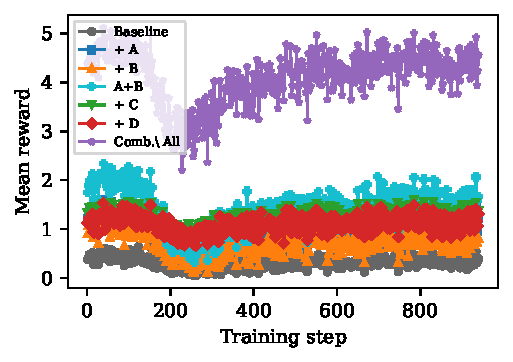
\includegraphics[width=\textwidth]{component/figures/p4/fig_reward_curves.pdf}
\caption{Mean total reward over training steps for all four pre-P3 runs.}
\label{fig:p4-reward-curves}
\end{figure}

The baseline (correctness only) peaks at step 124 (reward 0.641) then declines to 0.391 by the end of training, close to its starting value of 0.375.
Separate A peaks earlier (step 39) but sustains a higher correctness component throughout training, ending at 0.422 vs.\ the baseline's 0.391.
Separate B peaks at step 152 but its correctness component actually declines below the starting value by training end (0.348), suggesting the proximity reward may interfere with correctness optimization over long training horizons.
Combined A+B peaks at step 39, matching Separate A's early peak timing, and ends with the highest correctness component (0.418).

\paragraph{Per-component rewards.}
Figure~\ref{fig:p4-components} shows the individual reward components for the combined A+B run.

\begin{figure}[H]
\centering
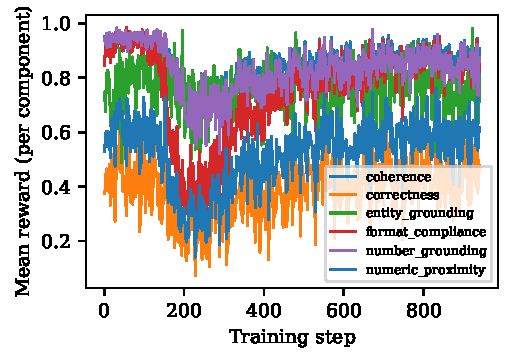
\includegraphics[width=\textwidth]{component/figures/p4/fig_component_rewards.pdf}
\caption{Per-component reward curves for the Combined A+B run. Correctness, format compliance, and numeric proximity are tracked separately.}
\label{fig:p4-components}
\end{figure}

In the combined run, format compliance starts high (0.844) reflecting the SFT checkpoint's existing formatting ability, while correctness starts low (0.375).
By training end, correctness improves to 0.418, format compliance decreases slightly to 0.715, and numeric proximity remains relatively stable (0.531 $\to$ 0.534).
The stability of numeric proximity suggests it provides a consistent background signal rather than driving active optimization.

\paragraph{Sequence length.}
Figure~\ref{fig:p4-seq-length} shows mean response length trends.

\begin{figure}[H]
\centering
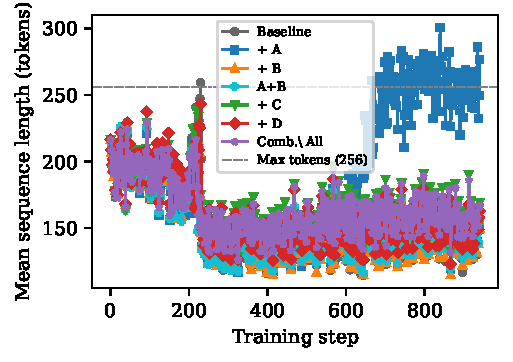
\includegraphics[width=\textwidth]{component/figures/p4/fig_seq_length.pdf}
\caption{Mean sequence length over training steps for all four pre-P3 runs.}
\label{fig:p4-seq-length}
\end{figure}

A notable divergence emerges: Separate A's sequence length increases from 216.5 to 276.6 tokens, while all other runs decrease (baseline: 216.5 $\to$ 148.3, Separate B: 216.5 $\to$ 150.1, Combined A+B: 216.5 $\to$ 154.6).
The format compliance reward appears to incentivize longer responses in isolation---likely because longer responses have more opportunities to include the \texttt{\#\#\#\#} marker.
When combined with other rewards (A+B), this effect is suppressed, and the model follows the same shortening trend as the baseline.
No runs exhibit sequence collapse (very short responses) or extreme length exploitation, indicating stable training behavior.
